

\subsection{Время рендеринга}


\begin{figure}
    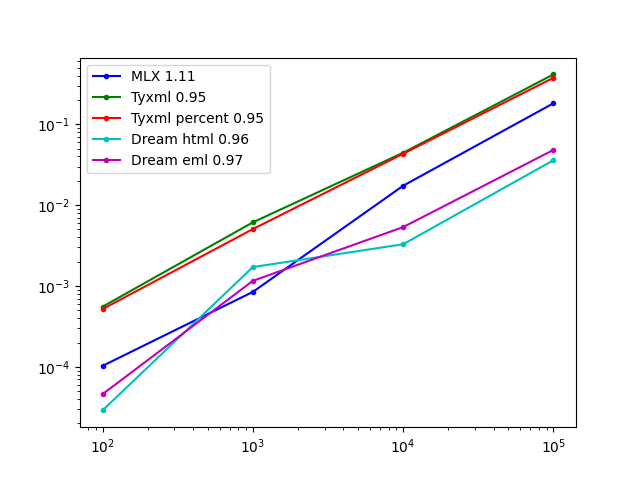
\includegraphics[width=\textwidth]{perfomance.png}
    \label{fig:perfomance}
    \caption{Сравнение производительности шаблонизаторов. График построен с помощью пакета matplotlib. Числа в легенде соответствуют аппроксиммированному углу наклона прямых. Масштаб выбран логарифмическим}
\end{figure}

EML показал наихудший результат в сравнении с остальными шаблонизаторами.
По показателям выделения памяти, выдвинута гипотеза о том, что проблема в чрезмерном количестве аллокаций.

Любопытный пик также наблюдается вокруг значения 10 для фреймворка TyXML\%.
Дальнейшее исследование было произведено с меньшей гранулярностью.
График приведен на рисунке % // TODO \ref{fig:tyxml_perfomance}.
\begin{figure}
    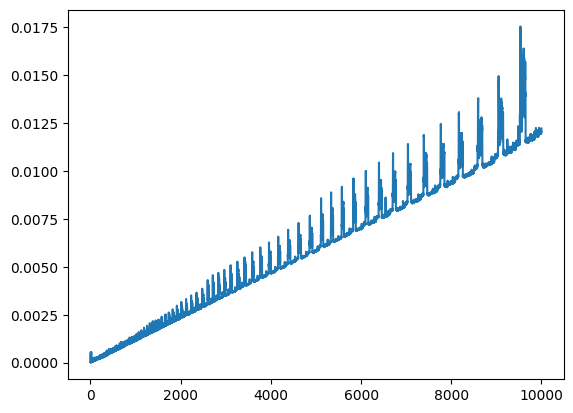
\includegraphics[width=\textwidth]{tyxml_performance.png}
    \label{fig:tyxml_perfomance}
    \caption{Время работы TyXML для тестов разных объемов. График построен с помощью пакета matplotlib}
\end{figure}

И TyXML и TyXML\% (в конце концов это один и тот же фреймворк) во время работы имеют пики с некоторой периодичностью.
Найденный ранее пик объясняется только удачей - если бы была выбрана другая гранулярность, пик мог быть утерян.
Предположительно, эти пики связаны с аллокацией памяти сборщиком мусора OCaml.
В рамках этой работы не были произведены дополнительные исследования этой аномалии\footnote{Обсуждение этой аномалии ведется на этом форуме https://discuss.ocaml.org/t/tyxml-performance/16776}. % // TODO: уточнить, можно ли так делать
